\chapter{Risultati}
\label{cap:3}
I risultati finali sono suddivisi nelle due caratteristiche su cui è stata sviluppata l'analisi dei dati.
Saranno presentate quindi una sezione relativa ai tempi di esecuzione e una sulla memoria fisica sfruttata. 
La descrizione delle relazioni più interessanti sarà, inoltre, accompagnata dall'utilizzo di alcuni tra i grafici elaborati durante lo studio statistico.

\section{Tempi di esecuzione}
L'indagine sui tempi di esecuzione, come spiegato nel paragrafo \ref{sbsec:Te}, è stata condotta approfondendo le seguenti relazioni: i tempi di esecuzione per le regole, la durata complessiva del processo e i tempi impiegati per intervalli differenti con lo stesso range. 
Questa sezione si occuperà di presentare gli esiti finali più rilevanti di ognuno di tali aspetti.

\subsection{Tempi e regole}
Le regole previste dal procedimento hanno concentrato l'analisi su due campi, una relativo a quei processi che non dipendono dal tipo di dati considerato e uno relativo a quelli che invece dipendono. 
Considerando le prime, è evidente dalla figura \ref{fig:Tind} come l'unico processo significativo è l'indicizzazione dello human reference per BWA, mentre le rimanenti non influiscono in alcun modo. 
In più, la differenza tra le potenze computazionali è netta già da questa figura, dato che tra l'apparecchio migliore e il peggiore vi è uno scarto di più di un'ora.
\begin{figure}[H]
\centering
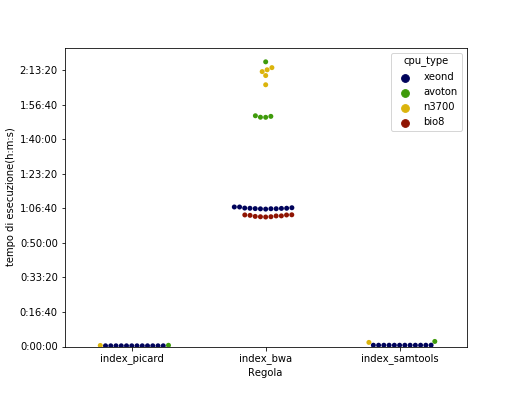
\includegraphics[scale=0.46]{Tind.png}
\caption{Tempi di esecuzione per le regole indipendenti dal subset.}
\label{fig:Tind}
\end{figure}
Nonostante la durata per l'indicizzazione sia già notevole, il vantaggio di questa fase  è che può essere riprodotta una sola volta per tutti i successivi lavori, visto che è riferita solamente al genoma umano di riferimento.

Passando alle regole dipendenti, i grafici riportati nella figura \ref{fig:Tdip} mostrano i vari andamenti per quei subset citati in precedenza con letture di range massimo 3 milioni.
Le fasi del procedimento che esauriscono più tempo sono la mappatura, che incrementa velocemente, e il riallineamento, che al contrario cresce lentamente; mentre le altre regole aumentano impiegando tempi sempre inferiori a 5 minuti.
\begin{table}[H]
  \begin{minipage}[b]{0.4\linewidth}
	\centering
	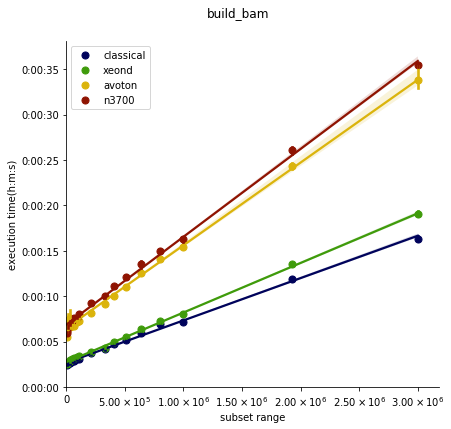
\includegraphics[width=1.33\textwidth]{build_bam.png}
	\captionof{figure}{Tempi per Build BAM.}
	\label{subfig:BB}
  \end{minipage}
  \hfill  
  \begin{varwidth}[b]{0.4\linewidth}
    \centering
	$\begin{array}{*{2}{c}}
		\toprule
			Nodo & Pendenza(\frac{s}{subset})\\
		\midrule
			\text{n3700} & 0.000010 \\
			\text{avoton} & 0.000009 \\
			\text{xeond} & 0.000006 \\
			\text{bio8} & 0.000005 \\
		\bottomrule
	\end{array}$
    \caption{Pendenze per i tempi di Build Bam.}
    \label{tab:Bb}
  \end{varwidth}%
\end{table}

\begin{table}[H]
  \begin{minipage}[b]{0.4\linewidth}
	\centering
	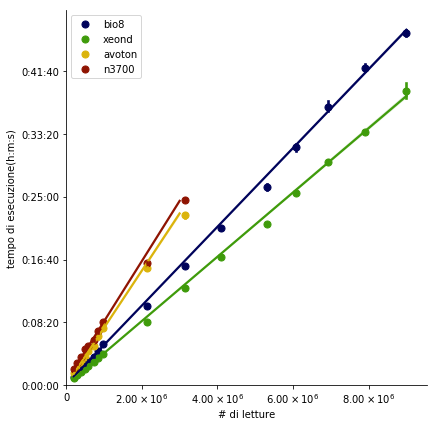
\includegraphics[width=1.33\textwidth]{mapping.png}	
	\captionof{figure}{Tempi per Mapping.}
	\label{subfig:Map}
  \end{minipage}
  \hfill  
  \begin{varwidth}[b]{0.4\linewidth}
    \centering
	$\begin{array}{*{2}{c}}
		\toprule
			Nodo & Pendenza(\frac{s}{subset})\\
		\midrule
			\text{n3700} & 0.000480 \\
			\text{avoton} & 0.000434 \\
			\text{xeond} & 0.000243 \\
			\text{bio8} & 0.000310 \\
		\bottomrule
	\end{array}$
    \caption{Pendenze per i tempi di Mapping.}
    \label{tab:Mp}
  \end{varwidth}%
\end{table}

\begin{table}[H]
  \begin{minipage}[b]{0.4\linewidth}
	\centering
	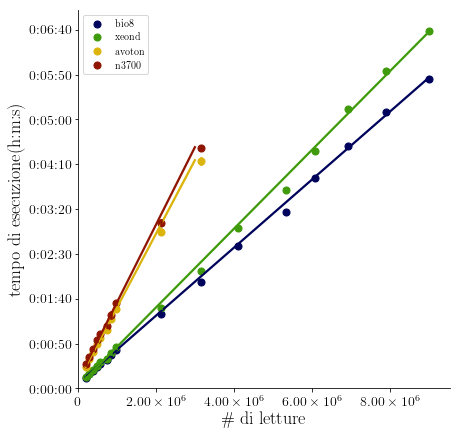
\includegraphics[width=1.33\textwidth]{mark_duplicates.png}
	\captionof{figure}{Tempi per Mark Duplicates.}
	\label{subfig:MD}
  \end{minipage}
  \hfill  
  \begin{varwidth}[b]{0.4\linewidth}
    \centering
	$\begin{array}{*{2}{c}}
		\toprule
			Nodo & Pendenza(\frac{s}{subset})\\
		\midrule
			\text{n3700} &  0.000088  \\
			\text{avoton} &  0.000082 \\
			\text{xeond} &  0.000042 \\
			\text{bio8} &  0.000040 \\
		\bottomrule
	\end{array}$
    \caption{Pendenze per i tempi di Mark Duplicates.}
	\label{tab:Md}
  \end{varwidth}%
\end{table}

\begin{table}[H]
  \begin{minipage}[b]{0.4\linewidth}
	\centering
	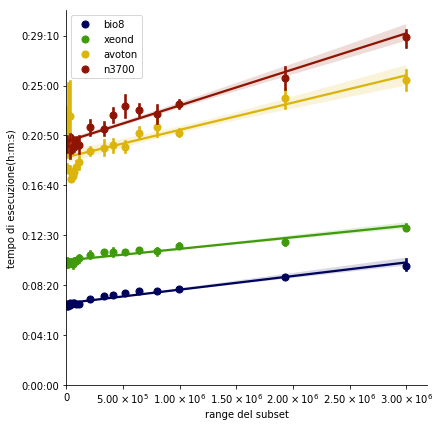
\includegraphics[width=1.33\textwidth]{realigner.png}
	\captionof{figure}{Tempi per i tempi di Realigner.}
	\label{subfig:Rlg}
  \end{minipage}
  \hfill  
  \begin{varwidth}[b]{0.4\linewidth}
	\centering
	$\begin{array}{*{2}{c}}
		\toprule
			Nodo & Pendenza(\frac{s}{subset})\\
		\midrule
			\text{n3700} &  0.000202 \\
			\text{avoton} &  0.000182 \\
			\text{xeond} & 0.000075 \\
			\text{bio8} & 0.000084 \\
		\bottomrule
	\end{array}$
    \caption{Pendenze per i tempi di Realigner.}
	\label{tab:Rlg}
  \end{varwidth}%
\end{table}

\begin{table}[H]
  \begin{minipage}[b]{0.4\linewidth}
	\centering
	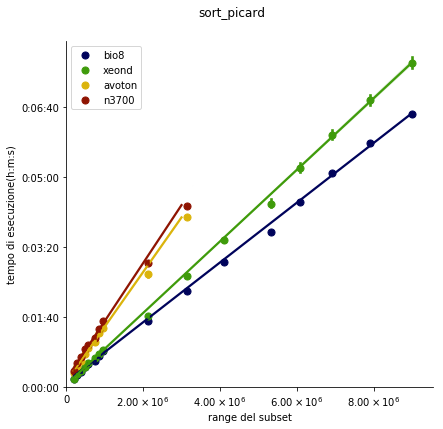
\includegraphics[width=1.33\textwidth]{sort_picard.png}
	\captionof{figure}{Tempi per i tempi di Sort Picard.}
	\label{subfig:SP}
  \end{minipage}
  \hfill  
  \begin{varwidth}[b]{0.4\linewidth}
    \centering
    	$\begin{array}{*{2}{c}}
		\toprule
			Nodo & Pendenza(\frac{s}{subset})\\
		\midrule
			\text{n3700} &   0.000089 \\
			\text{avoton} &  0.000080 \\
			\text{xeond} &  0.000052 \\
			\text{bio8} &  0.000048 \\
		\bottomrule
	\end{array}$
    \caption{Pendenze per i tempi di Sort Picard.}
    \label{tab:Sp}
  \end{varwidth}%
\end{table}


Ciascun gruppo di dati è stato sottoposto a regressione lineare e sono stati pure calcolati i coefficienti di correlazione, i quali hanno evidenziato come il tempo di esecuzione di ogni regola cresce linearmente rispetto al range del subset.
L'unica regola che mostra una particolarità è la fase di riallineamento(Figura\ref{subfig:Rlg}), dove soprattutto per la cpu Avoton i tempi oscillano quando i subset sono piccoli. 
In dettaglio, i coefficienti di correlazione in questo lavoro sono per le cpu Xeon, Atom(avoton) e Pentium n3700, rispettivamente: $0.812$, $0.656$ e $0.923$. 
Tale conseguenza è data da due fattori: l'oscillazione dei tempi per piccole variazioni del range e una caduta di performance dovute ad agenti scionosciuti, presumibilmente di natura tecnica.
Quest'ultimo effetto è rilevabile visibilmente per avoton nel grafico \ref{subfig:Rlg}, dove il fenomeno di oscillazione iniziale è ben nitido.
Nonostante ciò, visto che il numero di dati è abbondantemente superiore al centinaio, il coefficiente di Pearson determina che sia comunque altamente probabile una disposizione lineare per i dati.



%\'E possibile visualizzare grazie al grafico () l'andamento della macchina più performante, nominata xeond, rispetto ad un esempio di macchina tradizionale, classical, sull'intero range da 0 a 9 milioni.


\subsection{Durata complessiva}
Un altro aspetto rilevato è stato il tempo complessivo richiesto per svolgere tutti i passaggi che dipendono dal subset, quindi escludendo soprattuto l'indicizzazione per bwa.
Il grafico \ref{fig:Ttot} è riferito ai subset con massimo range di 3 milioni e, anche in questo caso, la regressione lineare è confermata dai coefficienti di correlazione che superano abbondantemente lo $0.95$, per ciascuna macchina.

\begin{table}[H]
  \begin{minipage}[b]{0.4\linewidth}
	\centering
	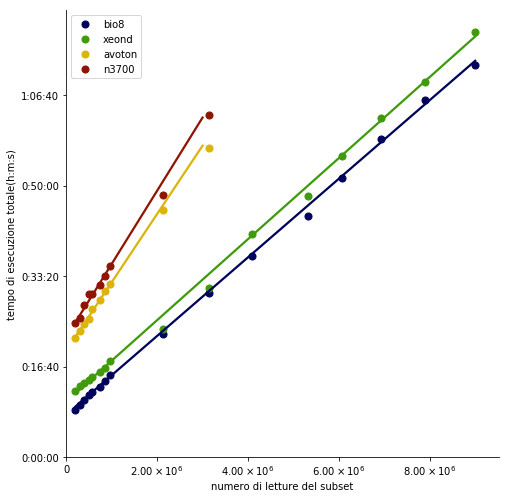
\includegraphics[width=1.33\textwidth]{Tempi_complessivi.png}	
	\captionof{figure}{Tempi complessivo di esecuzione.}
	\label{fig:Ttot}
  \end{minipage}
  \hfill  
  \begin{varwidth}[b]{0.4\linewidth}
    \centering
	$\begin{array}{*{2}{c}}
		\toprule
			Nodo & Pendenza(\frac{s}{subset})\\
		\midrule
			\text{n3700} & 0.000869 \\
			\text{avoton} & 0.000803 \\
			\text{xeond} & 0.000424 \\
			\text{bio8} & 0.000492 \\
		\bottomrule
	\end{array}$
    \caption{Pendenze per i tempi complessivi.}
    \label{tab:Ttot}
  \end{varwidth}%
\end{table}

\subsection{Tempi per stessi range}
Un approfondimento è stato richiesto per valutare quanto il contenuto dei dati influenzi la tenuta temporale e, di conseguenza, sono state considerate varie posizioni iniziali di estrazioni, dal materiale genetico grezzo, lasciando invariata la grandezza dei subset.
Questa operazione è stata fatta, come già indicato nel paragrafo \ref{subsec:simc}, su intervalli da diecimila e centomila numero di letture.

Sono riportati nella figura \ref{fig:Trng} due grafici rappresentativi dei due andamenti che predominano questa analisi.
\begin{figure}[H]
\centering
\subfloat[][\emph{Sort Picard per subset da diecimila reads.}]
	{\label{subfig:Spdieci}
	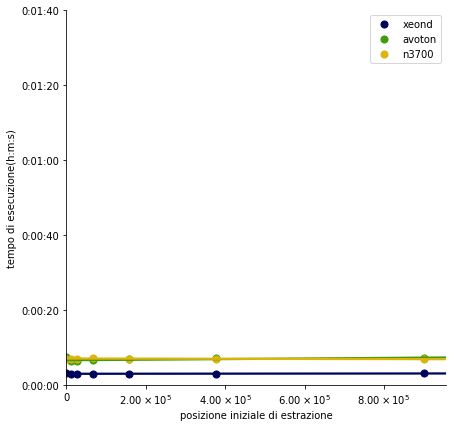
\includegraphics[width=.46\textwidth]{sort_picard_10000.png}
	} \quad
\subfloat[][\emph{Mapping per subset da centomila reads.}]
	{\label{subfig:Mcento}
	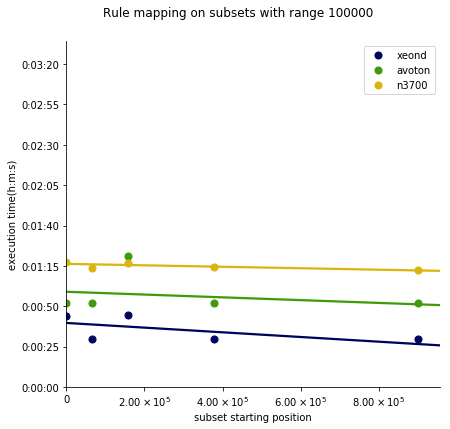
\includegraphics[width=.46\textwidth]{mapping_100000.png}
	} \\
\caption{}
\label{fig:Trng}
\end{figure}

Il primo caso è quello di un andamento costante, che si manifesta per la maggior parte dei grafici e che indica come le operazioni svolte dalla macchina non cambino in base alla diversità dei dati.
Il secondo rappresenta, invece, un andamento che si allontana dall'uniformità ma che assume più i contorni di un fenomeno stocastico rispetto al range del subset.
Dalla seconda figura si vede proprio l'effetto di allontanamento dalla retta di fit e già si vede come questa sia comunque leggermente inclinata senza un parvente motivo.

\'E possibile ipotizzare che per le regole che elaborano nello specifico le misure nei subset (la mappatura e il riallineamento), i lavori si adattino al tipo di dati e che ciò comporti un'oscillazione del tempo non ben prestabilita.

\section{Memoria utilizzata}
\textbf{rss-psutil}
La memoria occupata dai singoli processi è stata studiata analogamente al tempo, eccetto che per lo studio di una memoria complessiva per tutti i passaggi. 
Ciò implica che sono state analizzate in un primo momento le occupazioni della memoria per ognuna delle regole e che poi è stato tentato di definire l'andamento per diversi intervalli con stessa grandezza.
\'E indispensabile sottolineare che la memoria intesa in questo capitolo si riferisce alla memoria definita nel paragrafo \ref{subsubsec: SMb} "Resident Set Size", ricavata dal tool psutil e riportata da Snakemake. 

\subsection{Consumo di memoria per le regole}
Le informazioni sui vari comportamenti sono tratte dai grafici in figura \ref{fig:RSSr}, per i quali sono necessarie delle descrizioni specifiche, dato che non si ha un andamento generale. 
\begin{figure}[H]
\centering
\subfloat[][\emph{Memoria utilizzata da Build BAM.}]
	{\label{subfig:BB_rss}
	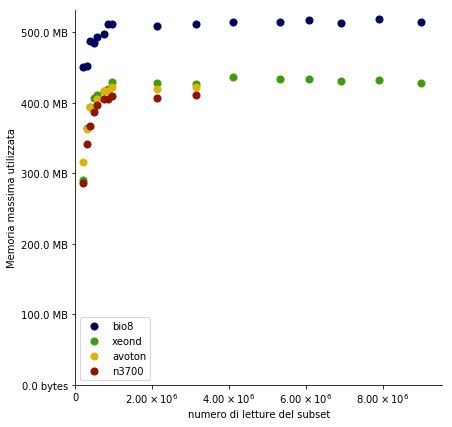
\includegraphics[width=.46\textwidth]{Max_rss_build_bam.png}
	} \quad
\subfloat[][\emph{Memoria utilizzata da Mapping.}]
	{\label{subfig:Map_rss}
	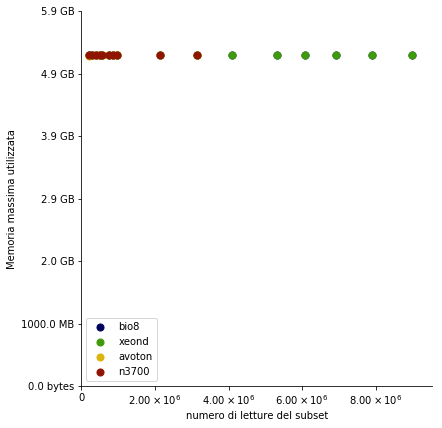
\includegraphics[width=.46\textwidth]{Max_rss_mapping.png}
	} \\
\end{figure}
\begin{figure}[H]
\ContinuedFloat
\centering
\subfloat[][\emph{Memoria utilizzata da Mark Duplicates.}]
	{\label{subfig:MD_rss}
	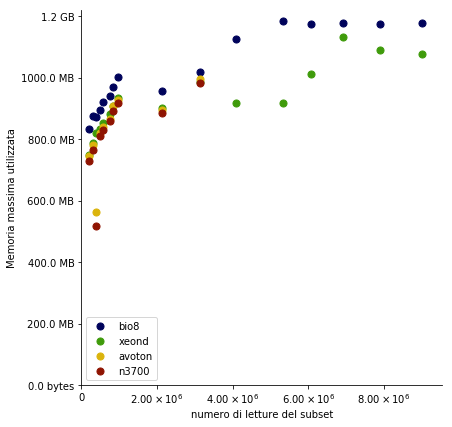
\includegraphics[width=.46\textwidth]{Max_rss_mark_duplicates.png}
	} \quad
\subfloat[][\emph{Memoria utilizzata da Realigner.}]
	{\label{subfig:Rlg_rss}
	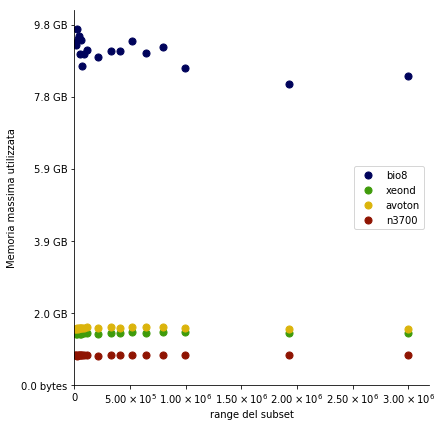
\includegraphics[width=.46\textwidth]{Max_rss_realigner.png}
	} \\
\end{figure}
\begin{figure}[H]
\ContinuedFloat
\centering
\subfloat[][\emph{Memoria utilizzata da Sort Picard.}]
	{\label{subfig:SP_rss}
	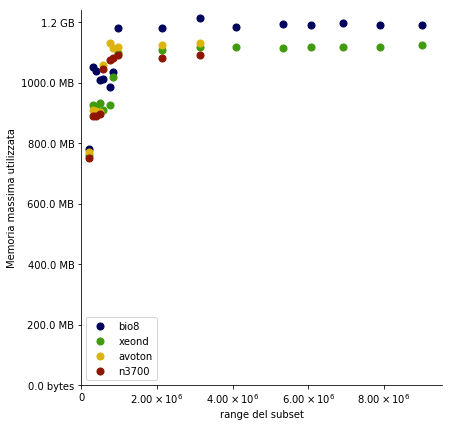
\includegraphics[width=.46\textwidth]{Max_rss_sort_picard.png}
	} 
\caption{}
\label{fig:RSSr}
\end{figure}

\'E evidente che regole di marcamento dei duplicati, di riordimento per picard e di formazione del file BAM, sono pressochè adattabili ad un logaritmo. 
Ciò indica una saturazione della memoria per un certo range di subset raggiunto e ciò è un fattore rilevante per la determinazione di un'uso efficace della parallelizzazione.

Le altre due regole che si soffermano specificatamente nei dati, la mappatura e il riallineamento, manifestano un valore fisso per l'uso della memoria ma in modalità distinte.
Nel caso del mapping, infatti, tutte le macchine lavorano alla stessa intensità, indicando una saturazione generale dell'utilizzo della memoria, mentre il riallineamento distingue per ognuna delle cpu valori inalterati differenti. 

Allo stesso modo che per i tempi, è stato ottenuto pure il grafico(\ref{fig:RSSind}) per le regole indipendenti dal set di dati, dove, a differenza di tale caso, anche l'indicizzazione dello human reference per picard consuma una parte della memoria.

\begin{figure}[H]
\centering
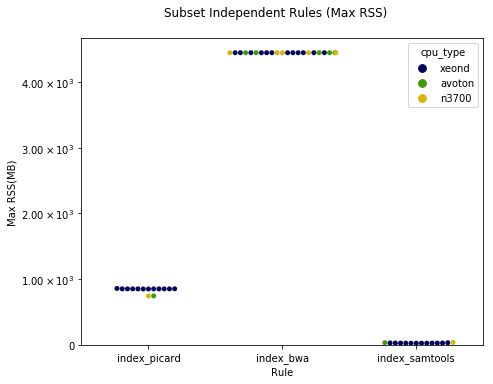
\includegraphics[scale=0.46]{Max_rss_ind.png}
\caption{Memoria utilizzate dalle regole indipendenti dai subsets.}
\label{fig:RSSind}
\end{figure}

\subsection{Memoria utilizzata per intervalli con stesso range}
Lo studio sulla memoria impiegata per intervalli diversi con stessi range ha prodotto due comportamenti caratteristici che sono stati posti in figura \ref{fig:RSSrng}.
\begin{figure}[H]
\centering
\subfloat[][\emph{Sort Picard per subset da diecimila reads.}]
	{\label{subfig:Spdiecirss}
	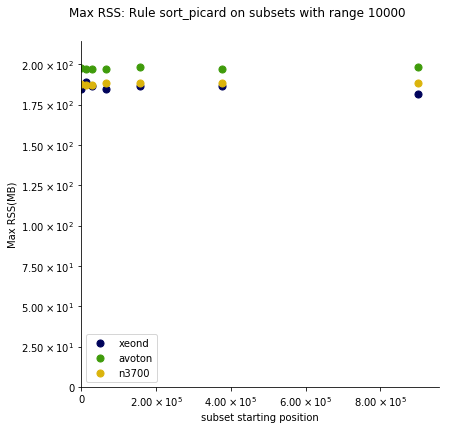
\includegraphics[width=.46\textwidth]{Max_rss_sort_picard_dieci.png}
	} \quad
\subfloat[][\emph{Mark Duplicates per subset da centomila reads.}]
	{\label{subfig:Mdcentorss}
	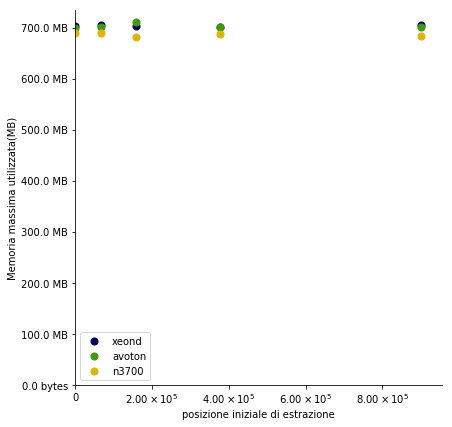
\includegraphics[width=.46\textwidth]{Max_rss_mark_duplicates_cento.png}
	} \\
\caption{}
\label{fig:RSSrng}
\end{figure}

Nella prima figura i dati oscillano leggermente intorno a valori fissi diversi per ciascuna cpu; mentre nella seconda, la linea su cui i dati si adattano è la stessa per tutti gli apparecchi.
Ciò indica come per alcuni lavori i dispositivi si comportino allo stesso modo e per altri invece la distinzione sia netta. 
In generale però, diversamente dai tempi di esecuzione, l'occupazione della memoria rss  per tutte le regole tende a non dipendere dal contenuto dei subset di ugual grandezza.

%\section{Processi di I-O} 
%Gli ultimi risultati sono stati ottenuti dall'indagine sui processi di input e output coinvolti nel completamento di ogni lavoro.
%Questa sezione, sugli stessi modelli precedenti, è stata suddivisa in due parti che determinano come la lettura e la scrittura sono dipendenti dal set di dati e se il contenuto di tali dati incide sull'uso della macchina.
%
%\subsection{I-O e regole}
%Il primo esito riportato è per le regole indipendenti dai subset ed a parte l'indicizzazione per BWA l'impatto è praticamente nullo.
%\begin{figure}[H]
%\centering
%\subfloat[][\emph{Scrittura per regole indipendenti dai subset}]
%	{\label{subfig:Iind}
%	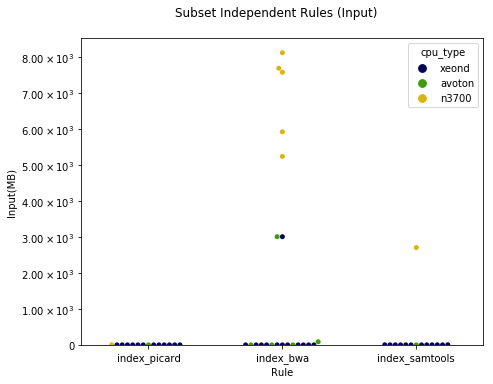
\includegraphics[width=.46\textwidth]{I_ind.png}
%	} \quad
%\subfloat[][\emph{Scrittura per regole indipendenti dai subset.}]
%	{\label{subfig:Oind}
%	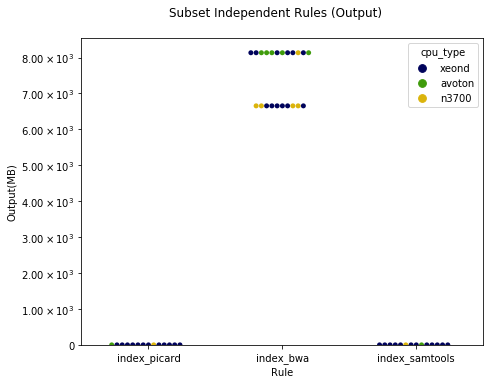
\includegraphics[width=.46\textwidth]{O_ind.png}
%	} \\
%\caption{}
%\label{fig:RSSrng}
%\end{figure}
%Diversamente dai tempi e dalla memoria, il lavoro di indicizzazione non è sempre costante sia per il caso di input che per quello dell'output.
%Riguardo all'input, le macchine più performanti (Xeon e Pentium N3700) nella maggior parte delle volte non eseguono alcuna lettura, mentre la rimanente varia in modo imprevedibile per valori elevati.
%Per l'output invece, l'andamento è costante per Pentium, al contrario di Xeon e Atom che similmente occupano due valori ben distinti. 
%
%
%Considerando le regole che invece dipendono dal subset, sono elecanti di seguito gli andamenti dei due processi per ognuna di esse.
%\begin{figure}[H]
%\centering
%\subfloat[][\emph{Lettura per la mappatura}]
%	{\label{subfig:IM}
%	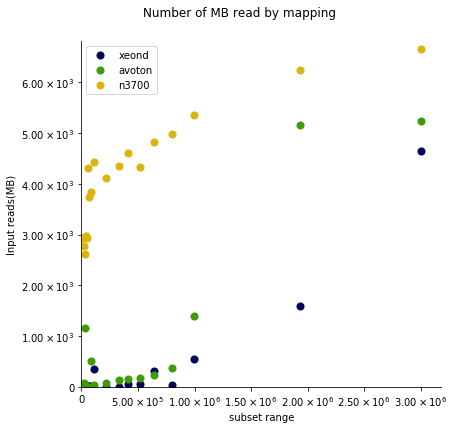
\includegraphics[width=.46\textwidth]{IO_Input_mapping.png}
%	} \quad
%\subfloat[][\emph{Scrittura per la mappatura}]
%	{\label{subfig:OM}
%	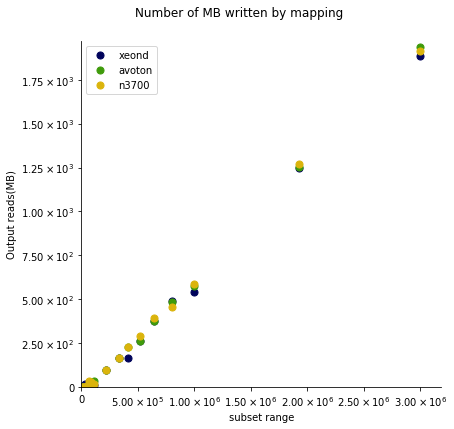
\includegraphics[width=.46\textwidth]{IO_Output_mapping.png}
%	} \\
%\caption{}
%\label{fig:IOm}
%\end{figure}
%
%La fase di lettura per la mappatura sembra crescere esponenzialmente per le due macchine migliori mentre per Pentium N3700 la crescita ha un andamento che tende a saturare in maniera logaritmica. 
%Gli elementi finali di Atom non seguono però un'esponenziale, suggerendo che avvenga una saturazione anche per le altre due macchine per grandezze dei subset superiori.
%
%La fase di scrittura, invece, mostra una andamento lineare praticamente omogeneo per tutte le macchine.  
%
%\begin{figure}[H]
%\centering
%\subfloat[][\emph{Lettura per il sorting di picard}]
%	{\label{subfig:ISp}
%	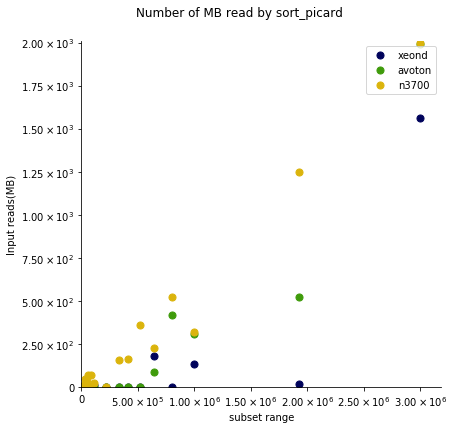
\includegraphics[width=.46\textwidth]{IO_Input_sort_picard.png}
%	} \quad
%\subfloat[][\emph{Scrittura per il sorting di picard}]
%	{\label{subfig:OSp}
%	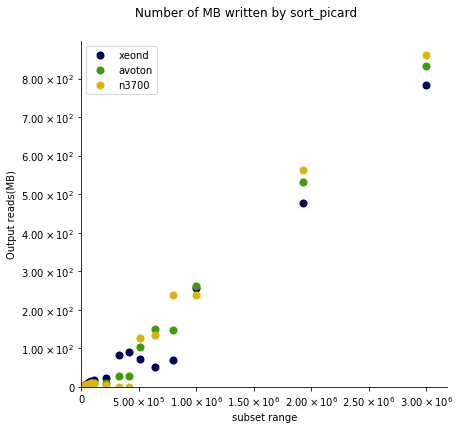
\includegraphics[width=.46\textwidth]{IO_Output_sort_picard.png}
%	} \\
%\caption{}
%\label{fig:IOSp}
%\end{figure}
%
%Per Picard il lavoro di riordinamento è ambiguo nella lettura perchè le macchine incrementano con traiettorie non ben definibili.
%Ad esempio, per Pentium la traiettoria potrebbe essere adattata ad una retta, ma esiste un certo sotto gruppo di dati che descrive una direzione nettamente diversa, così vanificando tale ipotesi.
%
%La scrittura invece inizia ad assumere contorni più chiari dopo una certa grandezza del subset, oltre il quale, tende a crescere linearmente. 
%Prima di raggiungere tale grandezza difatti ogni macchina, per range diversi, mostra un avvallamento non motivabile direttamente da questo tipo di studio statistico.  
%
%\begin{figure}[H]
%\centering
%\subfloat[][\emph{Lettura per la marcatura dei duplicati}]
%	{\label{subfig:IMd}
%	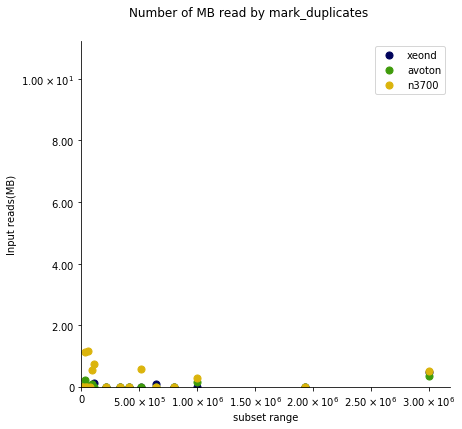
\includegraphics[width=.46\textwidth]{IO_Input_mark_duplicates.png}
%	} \quad
%\subfloat[][\emph{Scrittura per la marcatura dei duplicati}]
%	{\label{subfig:OMd}
%	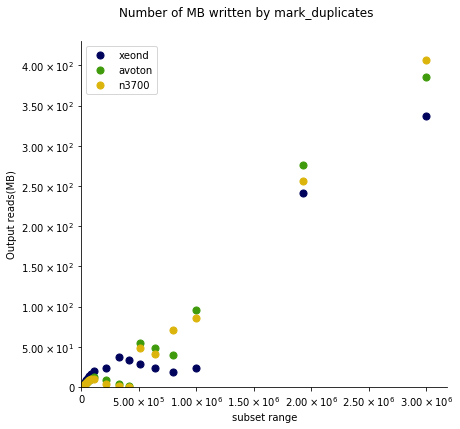
\includegraphics[width=.46\textwidth]{IO_Output_mark_duplicates.png}
%	} \\
%\caption{}
%\label{fig:IOMd}
%\end{figure}
%
%La descrizione della marcatura dei duplicati determina che la fase di lettura è coinvolta solo marginalmente, dato che esaurisce in generale meno di $2\,MB$, mentre quella di scrittura segue la stessa attitudine che il sorting per picard.
%Infatti ciò è evidente soprattutto in Xeon, per cui prima di avanzare con linearità è ben delineato un ventre di una curva.  
%
%\begin{figure}[H]
%\centering
%\subfloat[][\emph{Lettura per la formazione del BAM}]
%	{\label{subfig:IBB}
%	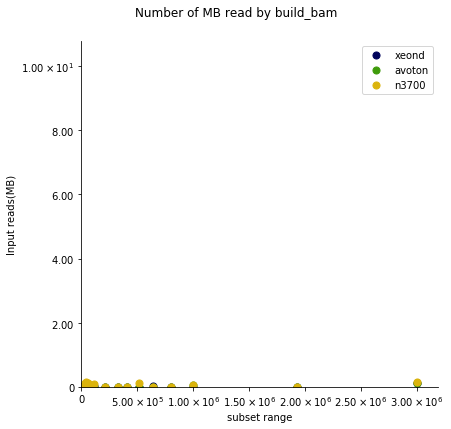
\includegraphics[width=.46\textwidth]{IO_Input_build_bam.png}
%	} \quad
%\subfloat[][\emph{Scrittura per la formazione del BAM}]
%	{\label{subfig:OBB}
%	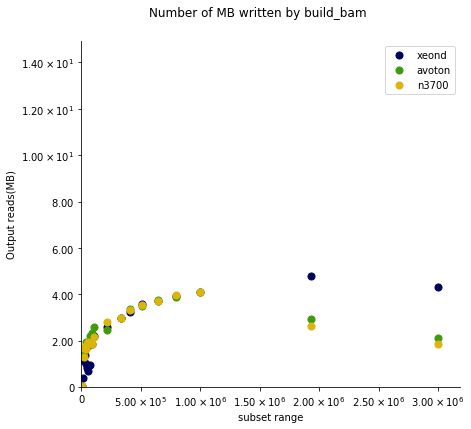
\includegraphics[width=.46\textwidth]{IO_Output_build_bam.png}
%	} \\
%\caption{}
%\label{fig:IOBB}
%\end{figure}
%
%Riguardo al passaggio per la costruzione dei file BAM, il numbero dei megabytes letti è trascurabile. 
%Al contrario, la scrittura segue una crescita logaritmica fino a circa 1 milione di subset, per poi cominciare a calare vistosamente.
%
%Le ragioni di questo calo non sono spiegabili, come nei casi precedenti, semplicemente osservando tale relazione dato che sarebbe più esauriente un approfindimento sia sulle prestazione dei macchinari che sul funzionamento dell'algoritmo di formazione del BAM. 
%
%\begin{figure}[H]
%\centering
%\subfloat[][\emph{Lettura per il riallineamento}]
%	{\label{subfig:IR}
%	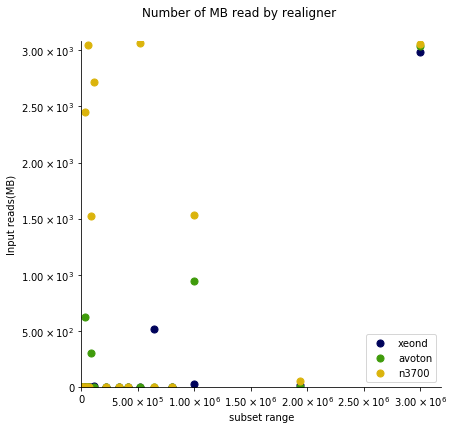
\includegraphics[width=.46\textwidth]{IO_Input_realigner.png}
%	} \quad
%\subfloat[][\emph{Scrittura per il riallineamento}]
%	{\label{subfig:OR}
%	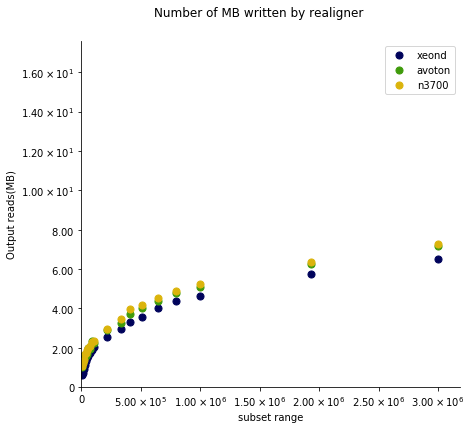
\includegraphics[width=.46\textwidth]{IO_Output_realigner.png}
%	} \\
%\caption{}
%\label{fig:IOR}
%\end{figure}
%
%In coda, il riallineamento mostra contemporaneamente il carattere meno comprensibile per la fase di lettura e quello più nitido per la fase di scrittura.
%I valori riportati nel grafico di input sono difficili da decifrare; non vi è un andamento univoco ne tra le cpu ne tra i dati associati ad ognuna di esse.
%Sono presenti un numero considerevole di processi che consumano una percentuale infinitesima in input che, però, sono alternati a salti elevati di letture, che tra loro non suggeriscono alcun andamento ben fissato.
%Evidentemente la natura del metodo di riallineamento influenza pesantemente questa fase di scansione dei bytes, riproducendo una lettura di essi fortemente discontinua.
%
%Nettamente diverso è il caso della scrittura, dove i dati tracciano una curva simile ad un logaritmo senza essere dotati di valori estranei ad essa.
%In più, i vari andamenti sono ordinati rispetto alla potenza computazionale delle macchine anche se, in questo frangente, con discrepanze molto sottili.
%
%\par Prima di passare al caso degli intervalli diversi con stesso intervallo, è utile sottolineare quali sono i lavori che generalemente consumano più bytes in fase di lettura e scrittura.
%In entrambi i casi è il mapping che vanta l'utilizzo maggiore e, all'opposto, è la formazione dei BAM che necessita del minor uso delle operazioni di input e output. 
%L'unico passaggio che presenta una netta inversione nell'uso di lettura e scrittura è, come si può controllare in figura \ref{fig:IOR}, il riallineamento, per cui sarà necessario uno studio specifico.
%
%\subsection{I-O per stessi range}
%L'ultima valutazione è stata eseguita, allo stesso modo che per i tempi e la memoria,  su intervalli diversi con lo stesso numero di letture.
%Sono stati scelti i grafici sottostanti per illustrare gli andamenti più interessanti ricavati durante le analisi.
%\begin{figure}[H]
%\centering
%\subfloat[][\emph{Input per realigner su range diecimila}]
%	{\label{subfig:IRdieci}
%	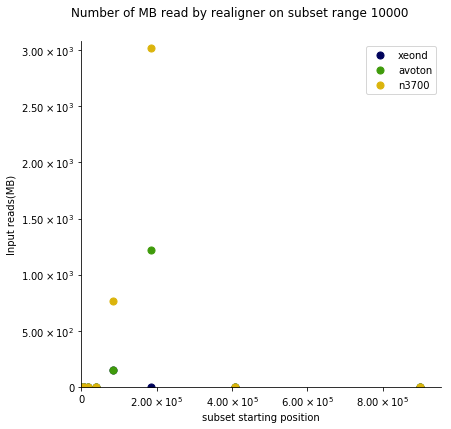
\includegraphics[width=.46\textwidth]{IO_I_realigner_dieci.png}
%	} \quad
%\subfloat[][\emph{Output per realigner su range diecimila}]
%	{\label{subfig:ORdieci}
%	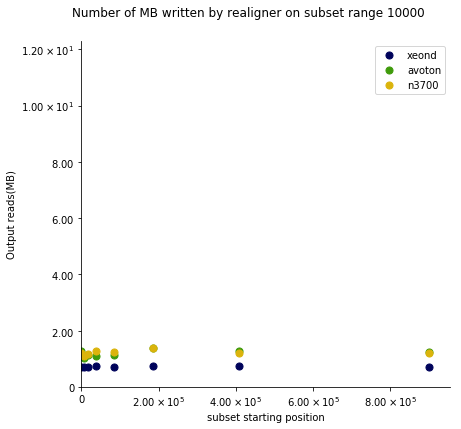
\includegraphics[width=.46\textwidth]{IO_O_realigner_dieci.png}
%	} \\
%\end{figure}
%\begin{figure}[H]
%\ContinuedFloat
%\centering
%\subfloat[][\emph{Input per mapping su range centomila}]
%	{\label{subfig:MIcento}
%	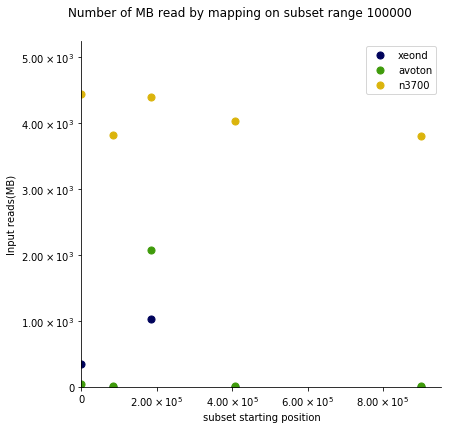
\includegraphics[width=.46\textwidth]{IO_I_map_cento.png}
%	} \quad
%\centering
%\subfloat[][\emph{Output per mapping su range centomila}]
%	{\label{subfig:MOcento}
%	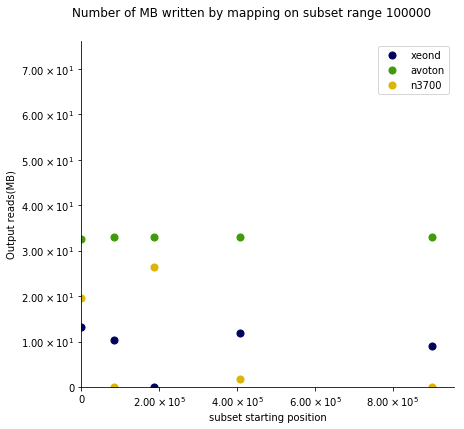
\includegraphics[width=.46\textwidth]{IO_O_map_cento.png}
%	} 
%\caption{}
%\label{fig:IOrng}
%\end{figure}
%
%I passaggi di scrittura mostrano un andamento più omogeneo per tipo di subset, pressochè costante nel caso della figura \ref{subfig:ORdieci} e per Atom(avoton) in \ref{subfig:ORdieci}.
%\'E interessante notare come le macchine computino con modalità diverse e che ciò causi la perdita dell'ordine delle cpu, dalla migliore alla peggiore, che caratterizzava le analisi per i tempi e la memoria.  
%
%Diverso è il caso della lettura che è rappresentato sia in \ref{subfig:IRdieci} che in \ref{subfig:MIcento}.  
%Le varie tracce non seguono andamenti ben definiti e sono spesso accompagnati da netti salti tra le misure di lettura, i quali inducono a pensare che sia il contenuto dei subset a determinare il tipo di lettura da svolgere. 
